La figura mostra la gràfica d'una funció $f$. La recta discontínua és una asímptota
vertical; els cercles buits indiquen punts que no pertanyen a la gràfica i els cercles
plens, punts que sí que hi pertanyen.

\begin{center}
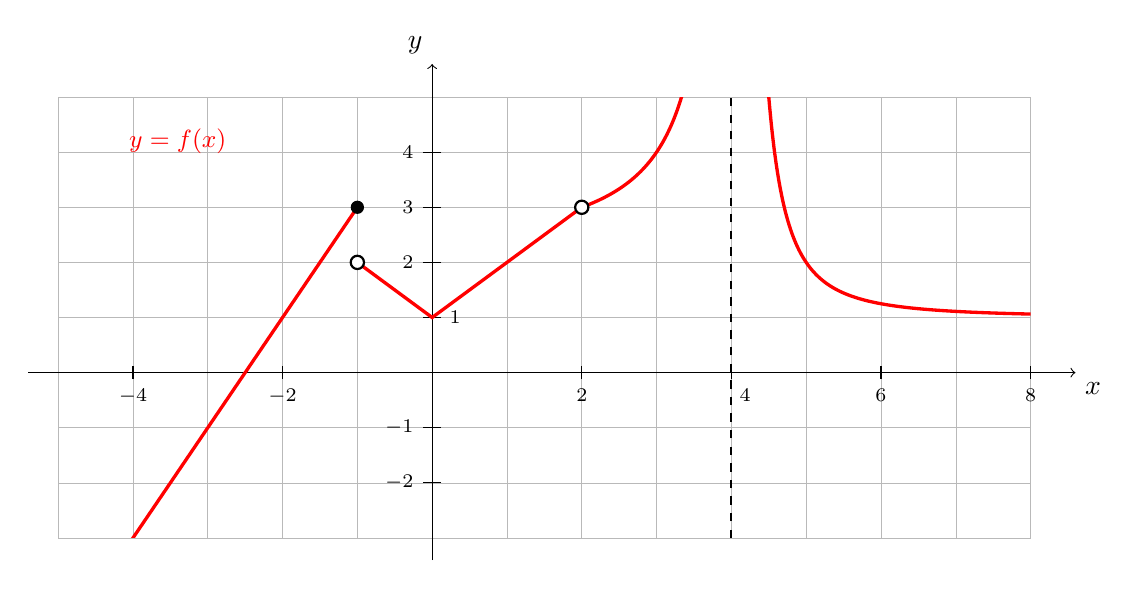
\begin{tikzpicture}[x=0.95cm,y=0.7cm]
  % Branques:  2x+5 (x<=-1) | |x|+1 (-1<x<2) | 2+2/(4-x) (2<x<4) | 1+1/(x-4)^2 (x>4)
  \draw[gray!55,very thin,step=1] (-5,-3) grid (8,5);
  \draw[->] (-5.4,0) -- (8.6,0) node[below right] {$x$};
  \draw[->] (0,-3.4) -- (0,5.6) node[above left] {$y$};
  \foreach \i in {-4,-2,2,6,8} \draw (\i,0.12) -- (\i,-0.12) node[below,font=\scriptsize] {$\i$};
  \draw (4,0.12) -- (4,-0.12) node[below,xshift=5pt,font=\scriptsize] {$4$};
  \foreach \j in {-2,-1,2,3,4} \draw (0.12,\j) -- (-0.12,\j) node[left,font=\scriptsize] {$\j$};
  \draw (0.12,1) -- (-0.12,1) node[right,xshift=6pt,font=\scriptsize] {$1$};
  \draw[dashed,thick] (4,-3) -- (4,5);
  \begin{scope}
    \clip (-5,-3) rectangle (8,5);
    \draw[red,very thick] (-5,-5) -- (-1,3);
    \draw[red,very thick] (-1,2) -- (0,1) -- (2,3);
    \draw[red,very thick,domain=2:3.6,samples=80,smooth] plot (\x,{2+2/(4-\x)});
    \draw[red,very thick,domain=4.35:8,samples=100,smooth] plot (\x,{1+1/((\x-4)^2)});
  \end{scope}
  \fill (-1,3) circle (2.4pt);
  \draw[fill=white,thick] (-1,2) circle (2.4pt);
  \draw[fill=white,thick] (2,3) circle (2.4pt);
  \node[red,font=\small] at (-3.4,4.2) {$y=f(x)$};
\end{tikzpicture}
\end{center}

\begin{apartats}

\apartat{1,25}
A partir de la gràfica, determina el valor dels límits següents. Si algun no existeix,
indica-ho i justifica-ho amb els límits laterals.
\begin{graella}{4}
  \sa \lim_{x\to-\infty}f(x) & \sa \lim_{x\to-1^-}f(x) & \sa \lim_{x\to-1^+}f(x) & \sa \lim_{x\to-1}f(x)\\[10pt]
  \sa \lim_{x\to2}f(x) & \sa \lim_{x\to4^-}f(x) & \sa \lim_{x\to4}f(x) & \sa \lim_{x\to+\infty}f(x)
\end{graella}

\begin{solucio}
i) $-\infty$ \quad ii) $3$ \quad iii) $2$ \quad iv) no existeix, perquè els laterals
valen $3$ i $2$ \quad v) $3$ \quad vi) $+\infty$ \quad vii) $+\infty$, perquè els dos
laterals valen $+\infty$ \quad viii) $1$.
\end{solucio}

\apartat{1,25}
Indica, si existeixen, $f(-1)$, $f(0)$ i $f(2)$. Estudia la continuïtat de $f$ en
$x=-1$, $x=0$, $x=2$ i $x=4$, i classifica'n les discontinuïtats.

\begin{solucio}
$f(-1)=3$, $f(0)=1$ i $f(2)$ no existeix.\\
$x=-1$: $f(-1)=3$ coincideix amb el lateral esquerre, però el dret val $2$. Laterals
finits i diferents: \textbf{salt finit}.\\
$x=0$: $\lim_{x\to0}f(x)=1=f(0)$. \textbf{És contínua}: la gràfica hi fa un angle, però no
s'hi trenca. Continuïtat no vol dir suavitat.\\
$x=2$: $\lim_{x\to2}f(x)=3$, però $f(2)$ no existeix: \textbf{evitable}.\\
$x=4$: $f(4)$ no existeix i els dos laterals valen $+\infty$: \textbf{salt infinit}
(asímptota vertical $x=4$).
\end{solucio}

\end{apartats}
